Classical simulations of the non-variational QWOA would not be possible without HPC resources, which were provided by the Pawsey Supercomputing Centre. The simulations were performed using QuOp, a Python library for parallel simulation of quantum variational algorithms. \cite{QuOp_MPI_paper_variational,QuOp_MPI}

\section{Single Problem Instances}

A random graph with 10 nodes was generated using the Erdős-Rényi model with an edge probability of 0.5. One edge was then removed to create a second graph, slightly dissimilar to the first. The graphs are shown in Figure \ref{fig:graphs}. Using this construction, it is known that the optimal solution to the graph similarity problem is 0.98 (The adjacency matrices differ in two entries).

This construction was chosen because it is simple to implement and ensures that the graphs are similar, but not identical. Constructing graphs with high similarity is important to demonstrate the algorithm's ability to identify small differences between graphs, which is a key requirement for many practical applications of graph similarity, such as threat detection, social network analysis, or bioinformatics.

Since the space of permutations grows as $n!$, it becomes classically infeasible to simulate larger graphs. However, there is reason to believe the $n=10$ case is still illustrative of the algorithm's behaviour (the structure of the problem and the nature of the QWOA make it likely that similar patterns will emerge in larger instances). This $n=10$ case requires $10!=3,628,800$ permutations to be evaluated. Since every permutation corresponds to a unique basis state, this requires at least 22 qubits of storage on a quantum computer (since $2^{21} = 2,097,152 < 10! < 2^{22} = 4,194,304$).

The non-variational QWOA was simulated for 5 iterations. The initial and final probability distributions over the possible similarity scores are shown in figure \ref{fig:similarity_scores}. The initial distribution is approximately normal, centred around a similarity score of 0.5, which is expected since most permutations will yield a similarity score around this value. After 5 iterations of the algorithm, the distribution has shifted significantly towards higher similarity scores, with a pronounced peak at 0.7. This indicates that the algorithm has successfully concentrated probability mass on the optimal solution.

\begin{figure}
\centering
\begin{subfigure}{0.45\textwidth}
    \centering
    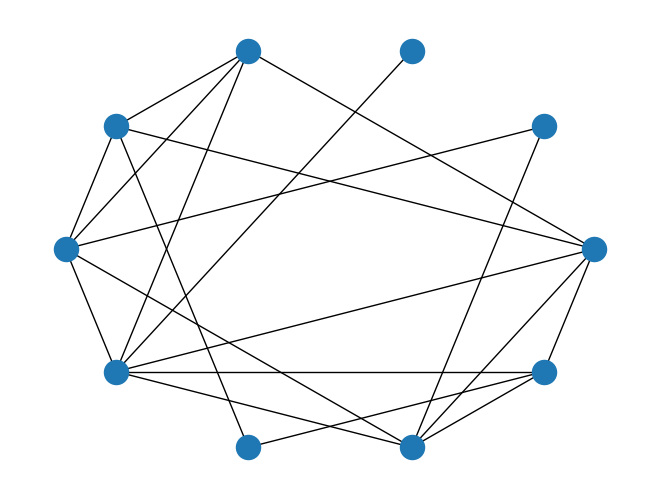
\includegraphics[width=\textwidth]{Figs/n=10_graph_1.png}
    \caption{Graph 1}
\end{subfigure}
\hfill
\begin{subfigure}{0.45\textwidth}
    \centering
    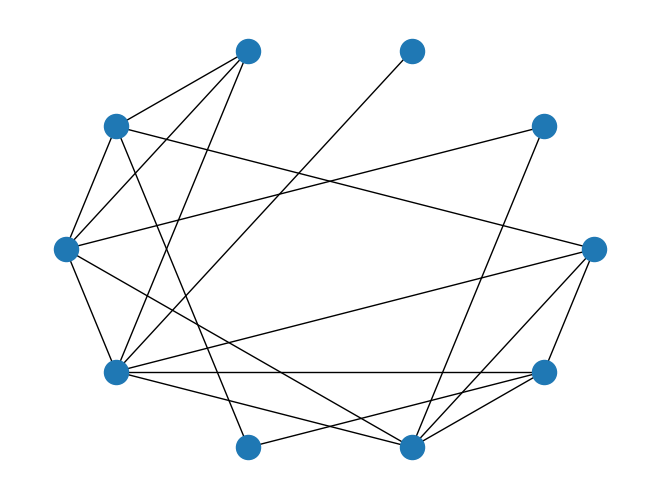
\includegraphics[width=\textwidth]{Figs/n=10_graph_2.png}
    \caption{Graph 2}
\end{subfigure}
\caption{The two graphs used in the first $n=10$ simulation. Graph 2 is derived from Graph 1 by removing one edge. Note that the nodes have been matched for visual clarity here, but node matching information is not available to the algorithm.}
\label{fig:graphs}
\end{figure}

\begin{figure}
\centering
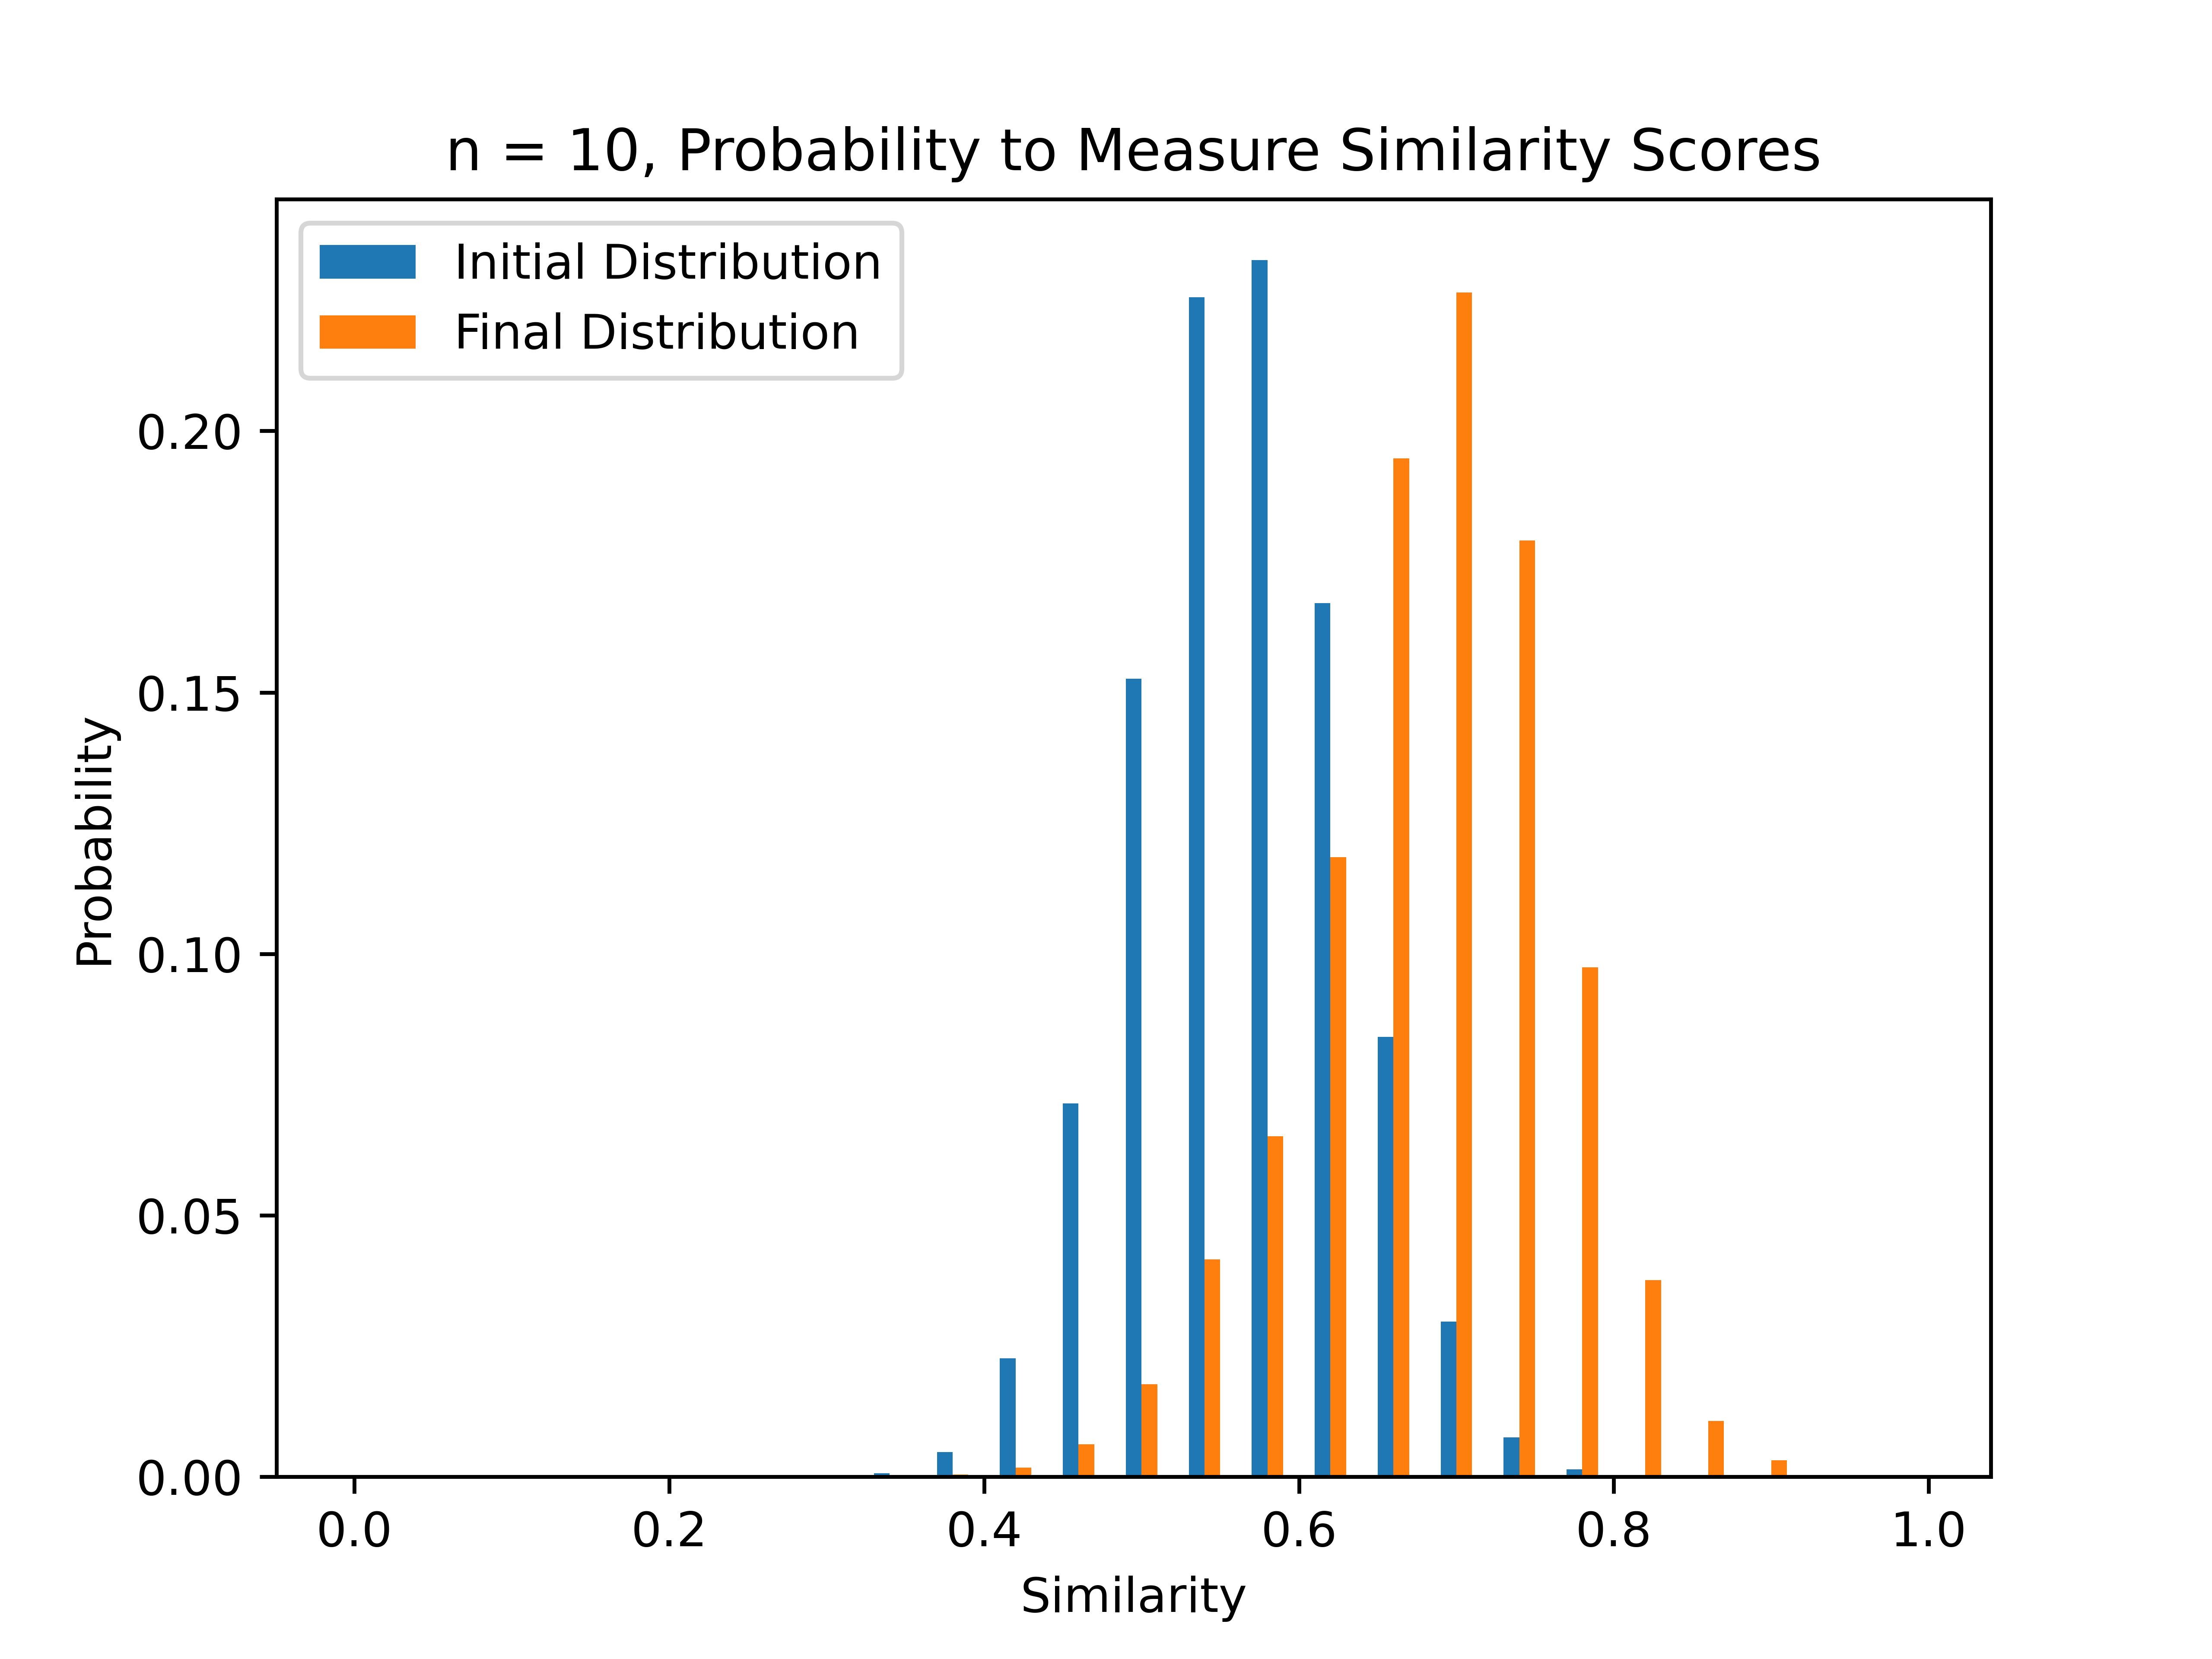
\includegraphics[width=0.5\textwidth]{Figs/n=10_Similarity_scores.png}
\caption{The initial and final probability distributions over similarity scores after 5 iterations of the non-variational QWOA for the $n=10$ case. The initial distribution is approximately normal, centred around a similarity score of 0.55. After 5 iterations, the distribution has shifted significantly towards higher similarity scores, with a pronounced peak at the optimal score of 0.7.}
\label{fig:similarity_scores}
\end{figure}

\section{Multiple Problem Instances}

Oh yeah.